\documentclass[11pt, letterpaper, twoside, tikz]{article}
\usepackage[letterpaper, portrait, left=1in, right=1in, top=1in, bottom=1in]{geometry}\usepackage{amsmath}
\usepackage{amssymb}
\usepackage{graphicx}
\usepackage[explicit]{titlesec}
\usepackage{epstopdf}
\usepackage{amsmath}
\usepackage{inputenc}
\usepackage{tikz}
\usetikzlibrary{babel}
\usetikzlibrary{arrows}
\usepackage{enumitem}
\title{MATH 270 Assignment 1}
\date{Athabasca University\\May 8, 2020}
\author{Stanley Zheng\and ID\# 3486740}
\usepackage{forest,mathtools,siunitx}
\makeatletter
\def\ifNum#1{\ifnum#1\relax
  \expandafter\pgfutil@firstoftwo\else
  \expandafter\pgfutil@secondoftwo\fi}
\forestset{
  num content/.style={
    delay={
      content/.expanded={\noexpand\num{\forestoption{content}}}}},
  pt@prime/.style={draw, circle},
  pt@start/.style={},
  pt@normal/.style={},
  start primeTree/.style={%
    /utils/exec=%
      % \pt@start holds the current minimum factor, we'll start with 2
      \def\pt@start{2}%
      % \pt@result will hold the to-be-typeset factorization, we'll start with
      % \pgfutil@gobble since we don't want a initial \times
      \let\pt@result\pgfutil@gobble
      % \pt@start@cnt holds the number of ^factors for the current factor
      \def\pt@start@cnt{0}%
      % \pt@lStart will later hold "l"ast factor used
      \let\pt@lStart\pgfutil@empty,
    alias=pt-start,
    pt@start/.try,
    delay={content/.expanded={$\noexpand\num{\forestove{content}}
                            \noexpand\mathrlap{{}= \noexpand\pt@result}$}},
    primeTree},
  primeTree/.code=%
    % take the content of the node and save it in the count
    \c@pgf@counta\forestove{content}\relax
    % if it's 2 we're already finished with the factorization
    \ifNum{\c@pgf@counta=2}{%
      % add the factor
      \pt@addfactor{2}%
      % finalize the factorization of the result
      \pt@addfactor{}%
      % and set the style to the prime style
      \forestset{pt@prime/.try}%
    }{%
      % this simply calculates content/2 and saves it in \pt@end
      % this is later used for an early break of the recursion since no factor
      % can be greater then content/2 (for integers of course)
      \edef\pt@content{\the\c@pgf@counta}%
      \divide\c@pgf@counta2\relax
      \advance\c@pgf@counta1\relax % to be on the safe side
      \edef\pt@end{\the\c@pgf@counta}%
      \pt@do}}

%%% our main "function"
\def\pt@do{%
  % let's test if the current factor is already greather then the max factor
  \ifNum{\pt@end<\pt@start}{%
    % great, we're finished, the same as above
    \expandafter\pt@addfactor\expandafter{\pt@content}%
    \pt@addfactor{}%
    \def\pt@next{\forestset{pt@prime/.try}}%
  }{%
    % this calculates int(content/factor)*factor
    % if factor is a factor of content (without remainder), the result will
    % equal content. The int(content/factor) is saved in \pgf@temp.
    \c@pgf@counta\pt@content\relax
    \divide\c@pgf@counta\pt@start\relax
    \edef\pgf@temp{\the\c@pgf@counta}%
    \multiply\c@pgf@counta\pt@start\relax
    \ifNum{\the\c@pgf@counta=\pt@content}{%
      % yeah, we found a factor, add it to the result and ...
      \expandafter\pt@addfactor\expandafter{\pt@start}%
      % ... add the factor as the first child with style pt@prime
      % and the result of int(content/factor) as another child.
      \edef\pt@next{\noexpand\forestset{%
        append={[\pt@start, pt@prime/.try]},
        append={[\pgf@temp, pt@normal/.try]},
        % forest is complex, this makes sure that for the second child, the
        % primeTree style is not executed too early (there must be a better way).
        delay={
          for descendants={
            delay={if n'=1{primeTree, num content}{}}}}}}%
    }{%
      % Alright this is not a factor, let's get the next factor
      \ifNum{\pt@start=2}{%
        % if the previous factor was 2, the next one will be 3
        \def\pt@start{3}%
      }{%
        % hmm, the previos factor was not 2,
        % let's add 2, maybe we'll hit the next prime number
        % and maybe a factor
        \c@pgf@counta\pt@start
        \advance\c@pgf@counta2\relax
        \edef\pt@start{\the\c@pgf@counta}%
      }%
      % let's do that again
      \let\pt@next\pt@do
    }%
  }%
  \pt@next
}

%%% this builds the \pt@result macro with the factors
\def\pt@addfactor#1{%
  \def\pgf@tempa{#1}%
  % is it the same factor as the previous one
  \ifx\pgf@tempa\pt@lStart
    % add 1 to the counter
    \c@pgf@counta\pt@start@cnt\relax
    \advance\c@pgf@counta1\relax
    \edef\pt@start@cnt{\the\c@pgf@counta}%
  \else
    % a new factor! Add the previous one to the product of factors
    \ifx\pt@lStart\pgfutil@empty\else
      % as long as there actually is one, the \ifnum makes sure we do not add ^1
      \edef\pgf@tempa{\noexpand\num{\pt@lStart}\ifnum\pt@start@cnt>1
                                           ^{\noexpand\num{\pt@start@cnt}}\fi}%
      \expandafter\pt@addfactor@\expandafter{\pgf@tempa}%
    \fi
    % setup the macros for the next round
    \def\pt@lStart{#1}% <- current (new) factor
    \def\pt@start@cnt{1}% <- first time
  \fi
}
%%% This simply appends "\times #1" to \pt@result, with etoolbox this would be
%%% \appto\pt@result{\times#1}
\def\pt@addfactor@#1{%
  \expandafter\def\expandafter\pt@result\expandafter{\pt@result \times #1}}

%%% Our main macro:
%%% #1 = possible optional argument for forest (can be tikz too)
%%% #2 = the number to factorize
\newcommand*{\PrimeTree}[2][]{%
  \begin{forest}%
    % as the result is set via \mathrlap it doesn't update the bounding box
    % let's fix this:
    tikz={execute at end scope={\pgfmathparse{width("${}=\pt@result$")}%
                         \path ([xshift=\pgfmathresult pt]pt-start.east);}},
    % other optional arguments
    #1
    % And go!
    [#2, start primeTree]
  \end{forest}}
\makeatother
\begin{document}
\begin{titlepage}
	\centering
	\vspace*{60px}
	\hspace{0pt}
	
\includegraphics[width=0.2\textwidth]{logo}\par\vspace{1cm}
	{\scshape\LARGE Athabasca University \par}
	\vspace{1cm}
	{\scshape\Large MATH 265\par}
	\vspace{1.5cm}
	{\huge\bfseries Assignment 1\par}
	\vspace{2cm}
	{\Large\itshape Stanley Zheng\par}
	\vfill
	{\large May 7, 2020\par}
	\vspace*{50px}
	\hspace{0pt}
\pagebreak
\end{titlepage}
\begin{enumerate}
\item
\begin{enumerate}[label=(\alph*)]
\item We can start by prime factoring the integer 220500.

\PrimeTree{220500}

We can then square root the prime factors and simplify.
$$\sqrt{2^2\times 3^2\times 5^3\times 7^2}=2\times3\times5\times7\sqrt{5}=\boxed{210\sqrt5}$$

\item Again, we can start by prime factorizing.

\PrimeTree{68600}

Next, we can cube root the factors of 68600 and simplify.
$$\sqrt[3]{2^3\times5^2\times7^3}=\boxed{14\sqrt[3]{25}}$$
\pagebreak
\item Again, we can start by prime factoring our two integers, 3267 and 4400.

\PrimeTree{3267}
\PrimeTree{4400}

Next, we can simplify each radical on its own.

$$3\sqrt[3]{11^2}\times 2^2\times5\times \sqrt{11}=3\times 11^{2/3}\times20\times 11^{1/2}$$

Since we can add the exponents of like terms when multiplying, our equation becomes

$$60\times 11 \times 11^{1/6}=\boxed{660\sqrt[6]{11}}$$

\item We can start by prime factorizing 1125 and 2420

\PrimeTree{1125}
\PrimeTree{2420}

Next, we can swap the prime factors into the radicals and simplify.

$$\sqrt{1125}+\sqrt{2420}=3\times 5\sqrt{5}+2\times 11\sqrt5=\boxed{37\sqrt5}$$

\end{enumerate}
\pagebreak
\item \hspace{50cm}%FIX THIS WHY IS THE NUMBER IN THE MIDDLE

\begin{tabular}{ |c|c|c| }
 \hline
 Interval & Inequality & Representation on the Real Line \\
 \hline
 $(-\infty,-1]$ & $x\leq -1$ & \raisebox{-\totalheight}{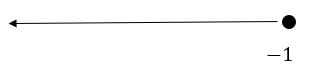
\includegraphics[width=0.2\textwidth]{Question1}}\\
 \hline
 $(\sqrt3, \infty)$ & $x>\sqrt3$ & \raisebox{-\totalheight}{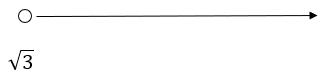
\includegraphics[width=0.2\textwidth]{Question2}}\\
 \hline
 $(-3, \pi)$ & $-3<x<\pi$ & \raisebox{-\totalheight}{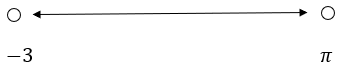
\includegraphics[width=0.2\textwidth]{Question3}}\\
 \hline
 $[\frac {3}{5}, \infty)$ & $\frac{3}{5}\leq x$ & \raisebox{-\totalheight}{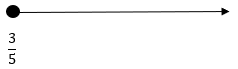
\includegraphics[width=0.2\textwidth]{Question4}}\\
 \hline
\end{tabular}
\item
\begin{enumerate}[label=(\alph*)]
\item $[-2, \infty)$ since the question specifies more than including negative two.
\item $(0,2]$ since the question specifies "and", we must choose the more restrictive interval.
\item $(3, \infty)$ since the question specifies "or", we must choose the less restrictive interval.
\end{enumerate}
\item
\begin{enumerate}[label=(\alph*)]
\item We can begin by simplifying the fraction inside of the parenthesis.
\begin{align*}
\left(\frac{5x^3yz^2}{xy^2z}\right)^{-\frac{3}{2}}&= (\frac{5x^2z}{y})^{-\frac{3}{2}}\\
&= \frac{y^{\frac{3}{2}}}{5^{\frac{3}{2}}x^3 z^{\frac{3}{2}}}
\end{align*}
\item We can start by expanding $(uv^2w^3-u^2w)^2$ and then multiplying by $v^{-2}$.
\begin{align*}
(uv^2w^3-3u^2w)^2(v^{-2})&= (u v^2 w^3-3u^2 w)\times(u v^2 w^3-3u^2w)\times(v^{-2})\\
&= (u^2v^4w^6-3u^3v^2w^4-3u^3v^2w^4+9u^4w^2)(v^{-2})\\
&=u^2v^2w^6-6u^3w^4+\frac{9u^4w^2}{v^2}
\end{align*}

\item We can start by converting all of the radicals into fractional exponents in order to make it easier to visualize and add.
\begin{align*}
(\sqrt{x^3}+x^2y^{-2}z)(xy^2z^3)&= (x^{\frac{3}{2}}+x^2y^{-2}z)(xy^2z^3)\\
&= x^{\frac{5}{2}}y^2z^3+x^3z^4
\end{align*}

\end{enumerate}
\item \begin{enumerate}[label=(\alph*)] %QUESTION 5 QUESTION 5
\item We can start by multiplying out the left side of the subtraction and the right side of the subtraction, then grouping like terms.
\begin{align*}
\sqrt{2}(3x-\sqrt2x^2+1)-\sqrt{18}(1-4x)^3&=(3\sqrt2x-\sqrt2\sqrt2x^2+1\sqrt2)-\sqrt{18}(1-4x)(16x^2-8x+1)\\
&=(3\sqrt2x-2x^2+\sqrt2)-\sqrt{18}(-64x^3+48x^2-12x+1)\\
&=(3\sqrt2x-2x^2+\sqrt2)-(-64\sqrt{18}x^3+48\sqrt{18}x^2-12\sqrt{18}+\sqrt{18})\\
\sqrt{18} \text { can be simplified into } 3\sqrt{2}\\
\end{align*}
$=(3\sqrt2x-2x^2+\sqrt2)-(-64\cdot 3\sqrt2x^3+48\cdot3\sqrt{2}x^2-12\cdot3\sqrt{2}+3\sqrt2)\\$
$=(3\sqrt2x-2x^2+\sqrt2)-(-192\sqrt{2}x^3+144\sqrt{2}x^2-36\sqrt{2}+3\sqrt{2})\\$
$=192\sqrt2x^3-144\sqrt2x^2-2x^2+39\sqrt2x-2\sqrt2$

\item We can begin by expanding the left side and right side of the addition sign, then grouping like terms.
\begin{align*}
(t-u)^2+5(3t-u+4u^2)(1+u)&=(t^2-2tu+u^2)+(4u^3+3u^2+3tu+3t-u)\\
&=(t^2-2tu+u^2)+(20u^3+15u^2+15tu+15t-5u)\\
&=20u^3+16u^2+t^2+13tu+15t-5u
\end{align*}

\item We can start by expanding the cubed trinomial, then multiplying by the binomial and grouping like terms.
\begin{align*}
(1-3x+x^2)^3(2-2x^2)&= (x^4-6x^3+11x^2-6x+1)(1-3x+x^2)(2-2x^2)\\
&= (x^6-9x^5+30x^4-45x^3+30x^2-9x+1)(2-2x^2)\\
&= -2x^8+18x^7-58x^6+72x^5-72x^3+58x^2-18x+2
\end{align*}

\end{enumerate}
\item \begin{enumerate}[label=(\alph*)]
\item We can factor by grouping like terms together
\begin{align*}
2y^3+6y^2+y+3&= 2y^2(y+3)+1(y+3)\\
&= (2y^2+1)(y+3)
\end{align*}
\item We can start by taking out a common factor of 3
\begin{align*}
3x^2-18xy+24y^2&= 3(x^2-6xy+8y^2)\\
&= 3(x-4y)(x-2y)
\end{align*}

\item Again, we can start by taking out a common factor of $2x$. The resulting trinonmial is a perfect square trinomial, so we factor it as such
\begin{align*}
50x^3+20x^2+2x&= 2x(25x^2+10x+1)\\
&= 2x(5x+1)^2
\end{align*}
\end{enumerate}
\item
\begin{enumerate}[label=(\alph*)]
\item We can start the simplification by factoring all polynomials and eliminating common factors from the fractions. Then, we can multiply both fractions to get a lowest common denominator
\begin{align*}
\frac{1}{9x^2-y^2}-\frac{12x^2-10xy+2y^2}{9x^2-6xy+y^2}&= \frac{1}{(3x+y)(3x-y)}-\frac{2(6x^2-5xy+y^2)}{(3x-y)^2}\\
&= \frac{1}{(3x+y)(3x-y)}-\frac{2(2x-y)(3x-y)}{(3x-y)^2}\\
&= \frac{1}{(3x+y)(3x-y)}-\left( \frac{2(2x-y)}{(3x-y)}\right) \left(\frac {3x+y}{3x+y}\right)\\
&= \frac{1}{(3x+y)(3x-y)}-\frac{2(2x-y)(3x+y)}{(3x-y)(3x+y)}\\
&= \frac {-12x^2+2xy+2y^2+1}{9x^2-y^2}
\end{align*}
\pagebreak
\item Similarly to the previous question, we can factor all polynomials and simplify the fractions.
\begin{align*}
\frac{\sqrt{x^2+5x+4}}{x^2+8x+16}-\frac{x^2-3x-4}{x^2-16}&= \frac{\sqrt{(x+4)(x+1)}}{(x+4)^2}-\frac{(x-4)(x+1)}{(x+4)(x-4)}\\
&= \frac{\sqrt{(x+4)(x+1)}}{(x+4)^2}-\frac{x+1}{x+4}\\
&= \frac{\sqrt{(x+4)(x+1)}}{(x+4)^2}-\left( \frac{x+1}{x+4}\right) \left( \frac{x+4}{x+4}\right)\\
&= \frac{-x^2-5x-4+\sqrt{x^2+5x+4}}{x^2+8x+16}
\end{align*}

\item Again, we factor all polynomials and simplify the fractions. However, since the operation between the fractions is now multiplication, we can eliminate factors across both fractions.
\begin{align*}
\left(\frac{9x^3+6x^2+x}{27x^3+1}\right)\left(\frac{6x-1}{3x^2+x}\right)&= \left( \frac{x(3x+1)^2}{(3x+1)(9x^2-3x+1)}\right) \left(\frac{6x-1}{x(3x+1)}\right)\\
&= \frac{6x-1}{9x^2-3x+1}
\end{align*}
\end{enumerate}
\item \begin{enumerate}[label=(\alph*)]

\item We can calculate the discriminant with the equation $b^2-4ac$. If the discriminant is 0, then there is 1 real solution. If the discriminant is more than 0, then the quadratic equation has 2 real solutions, and if the discriminant is less than 0, the quadratic equation has 2 complex solutions. Therefore, if the discriminant is more than 0, we can try to factor the quadratic equation or use the quadratic formula.

$$b^2-4ac=3^2-4(2)(-6)=57$$

This equation is not factorable, so we can use the quadratic formula.
\begin{align*}
x &= \frac{-b\pm \sqrt{b^2-4ac}}{2a}\\
x &= \frac{-3\pm \sqrt{3^2-4(2)(-6)}}{2\cdot 2}\\
x &= \frac{-3\pm \sqrt{57}}{4}
\end{align*}

\item Let $y=x^2$. Our equation becomes $y^2+6y-3=0$. Next, we can find the discriminant to see whether this quadratic equation has real solutions.

$$b^2-4ac=6^2-4(1)(-3)=48$$

Since this quadratic equation has 2 real solutions and is not factorable, we can use the quadratic formula.
\begin{align*}
y &= \frac{-b\pm \sqrt{b^2-4ac}}{2a}\\
y &= \frac{-6\pm \sqrt{6^2-4(1)(-3)}}{2\cdot 1}\\
y &= -3\pm2\sqrt3
\end{align*}

We substituted $y=x^2$ earlier, so we must substitute back $x^2=y$.
\begin{align*}
x^2 &= -3\pm2\sqrt3\\
x &= \pm\sqrt{\pm2\sqrt{3}-3}\\
\end{align*}
Since the question is asking only for real solutions, our two solutions are $\boxed {x=\pm\sqrt{2\sqrt3-3}}$

\item We can begin by moving all terms to one side.
$$12x^2-8x=0$$

It is immediately apparent that this equation can be factored into zero pairs, from which we can attain the roots.

$$4x(3x-2)=0$$

Looking at the zero pairs, our solutions are $\boxed{x=\frac{2}{3}, 0}$

\item We can start by multiplying by a lowest common multiple of 6 in order to eliminate the fractions, then finding the discriminant

$$2x^2+14x+15=0$$
$$b^2-4ac=14^2-4(2)(15)=76$$
Since the discriminant is positive, we know we have two real solutions. We can then plug the quadratic equation into the quadratic formula since it is not factorable.
\begin{align*}
x &= \frac{-b\pm \sqrt{b^2-4ac}}{2a}\\
x &= \frac{-14\pm \sqrt{14^2-4(2)(15)}}{2\cdot 2}\\
x &= \frac{-7\pm\sqrt19}{2}
\end{align*}

\item We can begin by multiplying by 2 to eliminate the fractions, then move all terms to one side and find the discriminant.

$$3x^2-2x+3=0$$
$$b^2-4ac=2^2-4(3)(3)=-32$$

Since the discriminant is negative, this quadratic equation has no real roots.
\end{enumerate}

\item \begin{enumerate}[label=(\alph*)]
\pagebreak
\item In order to rationalize this fraction, we can multiply both the numerator and denominator by the conjugate of the denominator, which in this case, is $5-\sqrt2$

\begin{align*}
\frac{\sqrt{2}-6}{5+\sqrt2}&= \left(\frac{2\sqrt6}{5+\sqrt2} \right)\left( \frac{5-\sqrt2}{5-\sqrt2}\right)\\
&= \frac{5\sqrt2-\sqrt2\times\sqrt2-30+6\sqrt2}{25-2}\\
&= \frac{11\sqrt2-32}{23}
\end{align*}

\item We can start by multiplying by the conjugate of the denominator.
\begin{align*}
\frac{5x-2}{\sqrt{2+x}-\sqrt{6x}}&= \left( \frac{5x-2}{\sqrt{2+x}-\sqrt{6x}}\right)\left( \frac{\sqrt{2+x}+\sqrt{6x}}{\sqrt{2+x}+\sqrt{6x}}\right)\\
&= \frac{5x\sqrt{2+x}+5x\sqrt{6x}-2\sqrt{2+x}-2\sqrt{6x}}{2+x-6x}
\end{align*}
To continue simplifying, we can factor the numerator by grouping like terms

\begin{align*}
\frac{5x\sqrt{2+x}+5x\sqrt{6x}-2\sqrt{2+x}-2\sqrt{6x}}{2+x-6x} &= \frac{5x)(\sqrt{2+x}+\sqrt{6x})-2(\sqrt{2+x}+\sqrt{6x})}{2-5x}\\
&= \frac{-(2-5x)(\sqrt{2+x}+\sqrt{6x})}{2-5x}\\
&= -\sqrt{2+x}-\sqrt{6x}
\end{align*}

\item We can start by multiplying by the conjugate of the denominator. Then, we can factor by grouping like terms and simplify the fraction.

\begin{align*}
\frac{\sqrt{8xy^3}+5\sqrt{y}}{2y-\sqrt{y}}&= \left(\frac{\sqrt{8xy^3}+5\sqrt {y}}{2y-\sqrt{y}} \right)\left( \frac{2y+\sqrt{y}}{2y+\sqrt{y}}\right)\\
&= \frac{2y\sqrt{8xy^3}+\sqrt{y}\sqrt{8xy^3}+5\times 2y\sqrt{y}+5\times \sqrt{y}\sqrt{y}}{(2y+\sqrt{y})(2y-\sqrt{y})}\\
&= \frac{\sqrt{8xy^3}(2+\sqrt{y})+5\sqrt{y}(2y+\sqrt{y})}{(2y+\sqrt{y})(2y-\sqrt{y})}\\
&= \frac{(2\sqrt{y}+1)(2y\sqrt{2x})+5}{4y-1}
\end{align*}
\end{enumerate}
\item \begin{enumerate}[label=(\alph*)]
\item We can start by adding the two fractions.
$$\frac{\pi}{5}+\frac{3\pi}{8}=\frac{8\pi}{40}+\frac{15\pi}{40}=\frac{23\pi}{40}$$
In order to convert from radians into degrees, we multiply by $\frac{180}{\pi}$.
\begin{align*}
\frac{23\pi}{40}\text{rad}&=\left( \frac{23\pi}{40}\right)\left( \frac{180^{\circ}}{\pi}\right)\\
&=\frac{4140^{\circ}}{40}\\
&=\boxed{\frac{207^{\circ}}{2}}
\end{align*}

\item We can start by multiplying by $\frac{180^{\circ}}{\pi}$
\begin{align*}
\frac{7\pi}{4}-\sqrt2\pi&\text{rad}= \left( \frac{7\pi}{4}-\sqrt{2}\pi\right)\left(\frac{180^{\circ}}{\pi}\right)\\
&=315^{\circ}-180\sqrt{2}^{\circ}
\end{align*}
\end{enumerate}
\item \begin{enumerate}[label=(\alph*)]
\item In order to convert from degrees to radians, we can multiply by $\frac{\pi}{180}$.

\begin{align*}
\left(\frac{38}{3}\right)^{\circ}&=\left(\frac{38}{3}\right)^{\circ}\left(\frac{\pi}{180}\right)\\
&=\frac{38\pi}{540}\\
&=\boxed{\frac{19\pi}{270}\text{rad}}
\end{align*}

\item Again, we can multiply by $\frac{\pi}{180}$. However, this time, the fraction $\frac{90}{5}$ can be reduced to 18.
\begin{align*}
\left(\frac{90}{5}\right)&=18^{\circ}\left(\frac{\pi}{180}\right)\\
&=\frac{18\pi}{180}\\
&=\boxed{\frac{1}{10}\text{rad}}
\end{align*}
\end{enumerate}
\item \begin{enumerate}[label=(\alph*)]

\item We can separate the fraction $\frac{7\pi}{6}$ into $\frac{\pi}{6}+\pi$. Since $\tan (a\pi+x)=\tan x$, we have
$$\tan \left(\frac{\pi}{6}\right)=\tan(30^{\circ})=\boxed{\frac{1}{\sqrt3}}$$

\item We can use the trigonometric identity of $\cos A \sin B=\frac{1}{2}(\sin (A+B)-\sin(A-B))$. Since we have $A=B$, our equation becomes $\frac{1}{2}\sin (\frac{5\pi}{4})$

The trigonometry unit circle shows that $\sin(\frac{5\pi}{4})=-\sin (\frac{\pi}{4})$. We know that $\sin (\frac{\pi}{4})=\frac{\sqrt2}{2}$. As a result, we have $\cos\left(\frac{5\pi}{8}\right)\sin\left(\frac{5\pi}{8}\right)=\boxed{-\frac{\sqrt2}{4}}$


\item We can use the trigonometric identity $\cos^2\theta=\frac{1+\cos(2\theta)}{2}$.
$$\frac{1+\cos(\frac{\pi}{4})}{2}$$
We know from the trigonometry unit circle that $\cos(\frac{\pi}{4})=\frac{\sqrt2}{2}$
Therefore, we have
$$\cos ^2\left(\frac{\pi}{8}\right)= \frac{1+\frac{\sqrt{2}}{2}}{2}=\boxed{\frac{\sqrt2+2}{4}}$$

\end{enumerate}
\item We can start by looking at the smaller triangle. Since the circle has a radius of 1, the hypotenuse of the smaller triangle is 1 unit long. We can call the $x$-axis side of the smaller triangle $a$ and the $y$-axis side of the smaller triangle $b$. Then, $a$ is $\cos \theta$, and $b$ is $\sin\theta$. Then, side $y$ on the big triangle is $z\sin \theta$ and side $x$ is $z\cos \theta$. Since the smaller triangle and the bigger triangle are similar triangles, they share the property that the ratio of corresponding sides are equal, as such
$$\frac{z}{1}=\frac{x}{a}=\frac{y}{b}$$
From here, we can substitute $a$ and $b$ for the functions defined earlier, and isolate for $\sin \theta$ and $\cos \theta$.
$$z=\frac{x}{\cos \theta}=\frac{y}{\sin \theta}$$
$$\cos \theta=\frac{x}{z} $$
$$\sin \theta=\frac{y}{z} $$

We know that $\tan \theta = \frac{\text{opposite}}{\text{adjacent}}$. However, when we divide the numerator and denominator by the hypotenuse, we get
$$\tan \theta=\frac{\text{(opposite)/(hypotenuse)}}{\text{(adjacent)/(hypotenuse)}}=\frac{\sin \theta}{\cos \theta}$$
Therefore, we have
$$\tan\theta=\frac{\frac{y}{z}}{\frac{x}{z}}=\frac{y}{x}$$

\end{enumerate}
\end{document}
